\let\lesson\undefined
\newcommand{\lesson}{\phantomlesson{Bài 12: Một số lực trong thực tiễn}}
\chapter[Lực cản và lực nâng của chất lưu]{Lực cản và lực nâng của chất lưu}
\setcounter{section}{0}
\section{Lý thuyết}
\subsection{Lực đẩy Archimedes}
Mọi vật chìm trong chất lưu (chất lỏng, không khí, \dots) đều chịu tác dụng của lực nâng. Lực nâng này được gọi là lực đẩy Archimedes và có đặc điểm như sau:
\begin{center}
	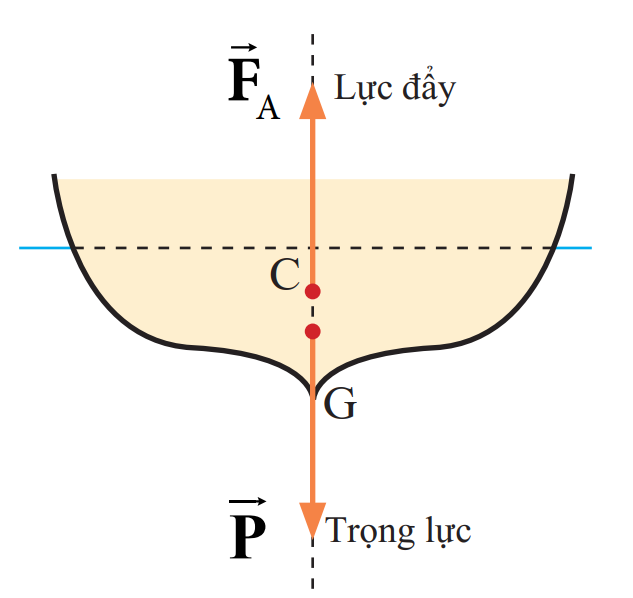
\includegraphics[width=0.25\linewidth]{../figs/VN10-2023-PH-TP020-1}
	\captionof{figure}{Trọng lực và lực đẩy Archimedes tác dụng lên vật.}
\end{center}
\begin{itemize}
	\item Điểm đặt: trọng tâm của phần chất lưu bị vật chiếm chỗ;
	\item Phương: thẳng đứng;
	\item Chiều: từ dưới lên trên;
	\item Độ lớn: bằng trọng lượng phần chất lưu bị vật chiếm chỗ
	$$F_A=\rho \cdot g \cdot V$$
	trong đó:
	\begin{itemize}
		\item $F_A$: độ lớn lực đẩy Archimedes tác dụng lên phần vật chìm $\left(\si{\newton}\right)$;
		\item $\rho$: khối lượng riêng của chất lưu $\si{\kilogram/\meter^3}$;
		\item $g$: gia tốc trọng trường $\si{\meter/\second^2}$;
		\item $V$: thể tích phần chất lưu bị vật chiếm chỗ $\si{\meter^3}$.
	\end{itemize}
\end{itemize}
\subsection{Áp suất chất lỏng}
\subsubsection{Định nghĩa áp suất}
Áp suất là đại lượng được xác định bằng độ lớn áp lực $F$ trên một đơn vị diện tích $S$ của mặt bị ép
$$p=\dfrac{F}{S}$$
Trong hệ SI, đơn vị của áp suất là $\si{\pascal}$ $\left(\SI{1}{\pascal}=\SI{1}{\newton/\meter^2}\right)$.\\
Trong chất lỏng luôn tồn tại áp suất do trọng lượng của chất lỏng tạo ra.
\subsubsection{Khối lượng riêng}
Khối lượng riêng của một chất là đại lượng được xác định bằng khối lượng $m$ của vật tạo thành từ chất đó trên một đơn vị thể tích $V$ của vật
$$\rho=\dfrac{m}{V}$$
Trong hệ SI, đơn vị của khối lượng riêng là $\si{\kilogram/\meter^3}$.
\subsubsection{Độ chênh lệch áp suất giữa hai điểm trong lòng chất lỏng}
Xét hai điểm $A$ và $B$ cách nhau một đoạn $\Delta h$ theo phương thẳng đứng trong chậu chứa một chất lỏng xác định. Độ chênh lệch áp suất giữa hai điểm $A$ và $B$
$$\Delta p=\rho \cdot g\cdot \Delta h$$
\subsection{Lực cản của chất lưu}
Khi chuyển động trong không khí, trong nước hoặc trong chất lỏng nói chung (gọi chung là chất lưu), vật đều chịu tác dụng của lực cản.
\begin{center}
	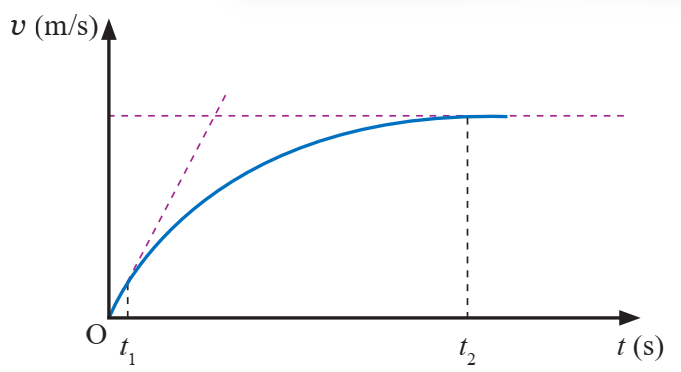
\includegraphics[width=0.4\linewidth]{../figs/VN10-2023-PH-TP020-2}
	\captionof{figure}{Đồ thị tốc độ theo thời gian của vật rơi trong chất lưu khi có lực cản.}
\end{center}
Chuyển động của vật trong chất lưu được chia thành 3 giai đoạn:
\begin{itemize}
	\item Nhanh dần đều từ lúc bắt đầu rơi trong một thời gian ngắn.
	\item Nhanh dần không đều trong một khoảng thời gian tiếp theo. Lúc này lực cản bắt đầu có độ lớn đáng kể và tăng dần.
	\item Chuyển động đều với tốc độ giới hạn không đổi. Khi đó, tổng hợp lực tác dụng lên vật rơi bị triệt tiêu.
\end{itemize}
\luuy{Sau khi vật chuyển động đều, nếu có thêm tác nhân làm tăng lực cản của chất lưu (ví dụ như người nhảy dù bung dù ra như trong Hình \ref{fig:20.3}), thì vật sẽ chuyển động chậm dần. Tốc độ rơi của vật giảm dần, lực cản cũng giảm đến khi tổng lực tác dụng lên vật lại bị triệt tiêu và vật trở lại trạng thái chuyển động đều.
\begin{center}
	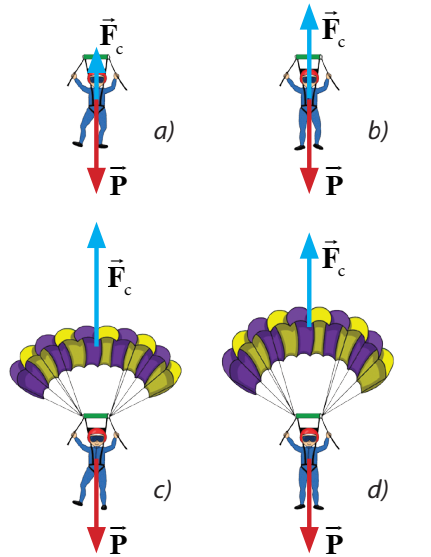
\includegraphics[width=0.4\linewidth]{../figs/VN10-2023-PH-TP020-3}
	\captionof{figure}{a) chưa bung dù; b) chuyển động ổn định khi chưa bung dù; c) vừa bung dù; d) chuyển động ổn định.}
	\label{fig:20.3}
\end{center}
}
Lực cản của chất lưu được biểu diễn bởi một lực đặt tại trọng tâm vật, cùng phương và ngược chiều với chiều chuyển động của vật trong chất lưu. Lực cản này phụ thuộc vào hình dạng và tốc độ của vật.
\section{Mục tiêu bài học - Ví dụ minh hoạ}
\begin{dang}{Thành lập và vận dụng được phương trình $\Delta p=\rho\cdot g\cdot\Delta h$ trong một số trường hợp đơn giản}
	\viduii{3}
	{Em hãy xây dựng biểu thức xác định độ chênh lệch áp suất giữa hai điểm có độ sâu khác nhau trong lòng chất lỏng.
}
{\hide{
Xét hai điểm $A$ và $B$ cách nhau một đoạn $\Delta h$ theo phương thẳng đứng trong chậu chứa một chất lỏng xác định. Giả định hai điểm $A$ và $B$ nằm trên hai mặt đáy của một bình chứa hình hộp chữ nhật tiết diện $S$, độ cao $\Delta h$ như Hình \ref{fig:20.4}.
\begin{center}
	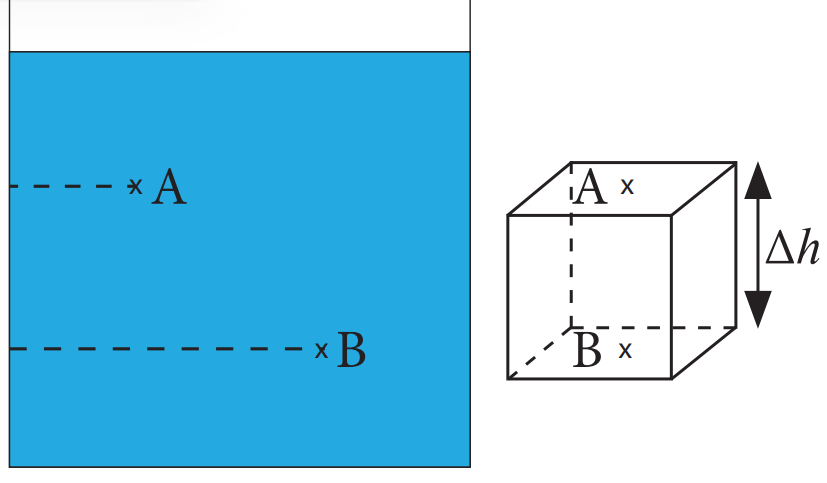
\includegraphics[width=0.3\linewidth]{../figs/VN10-2023-PH-TP020-4}
	\captionof{figure}{Hai điểm $A$ và $B$ trong lòng chất lỏng có thể được giả định thành hai điểm $A$ và $B$ nằm trên hai mặt đáy của một bình chứa hình hộp chữ nhật.}
	\label{fig:20.4}
\end{center}
Độ chênh lệch áp suất $\Delta p$ giữa hai đáy là do trọng lượng $mg$ của phần chất lỏng hình trụ có khối lượng $m$ gây ra trên một đơn vị diện tích. Theo định nghĩa áp suất, ta có
\begin{equation}
	\Delta p =\dfrac{mg}{S}
	\label{eq:20.1}
\end{equation}
Khối lượng của phần chất lỏng này được suy ra từ khối lượng riêng và thể tích của nó
$$m=\rho\cdot V=\rho \cdot S\cdot\Delta h$$
Thay vào biểu thức (\ref{eq:20.1}), ta có:
$$\Delta p=\rho\cdot g\cdot \Delta h$$
}}

\viduii{3}
{Kỉ lục thế giới về lặn tự do (không có bình dưỡng khí) được thực hiện bởi một nữ thợ lặn người Slovenia khi cô lặn xuống biển tới độ sâu $\SI{114}{\meter}$. Hãy tính độ chênh lệch áp suất tại vị trí này so với mặt thoáng của nước biển. Lấy giá trị trung bình khối lượng riêng của nước biển là $\SI{1025}{\kilogram/\meter^3}$ và $g=\SI{9.8}{\meter/\second^2}$.
}
{\hide{
Độ chênh lệch áp suất tại vị trí có độ sâu $\SI{114}{\meter}$ so với mặt thoáng của nước biển:
$$\Delta p=\rho g\Delta h=\left(\SI{1025}{\kilogram/\meter^3}\right)\cdot\left(\SI{9.8}{\meter/\second^2}\right)\cdot\left(\SI{114}{\meter}\right)\approx\SI{11.45E5}{\pascal}$$
}}
\end{dang}
\begin{dang}{ Mô tả được bằng ví dụ thực tiễn và biểu diễn được bằng hình vẽ: lực cản, lực nâng của chất lưu}
	\viduii{2}
	{Hãy vẽ lực cản của không khí hoặc nước tác dụng lên các vật trong các trường hợp được mô tả trong Hình \ref{fig:20.5}
		\begin{center}
			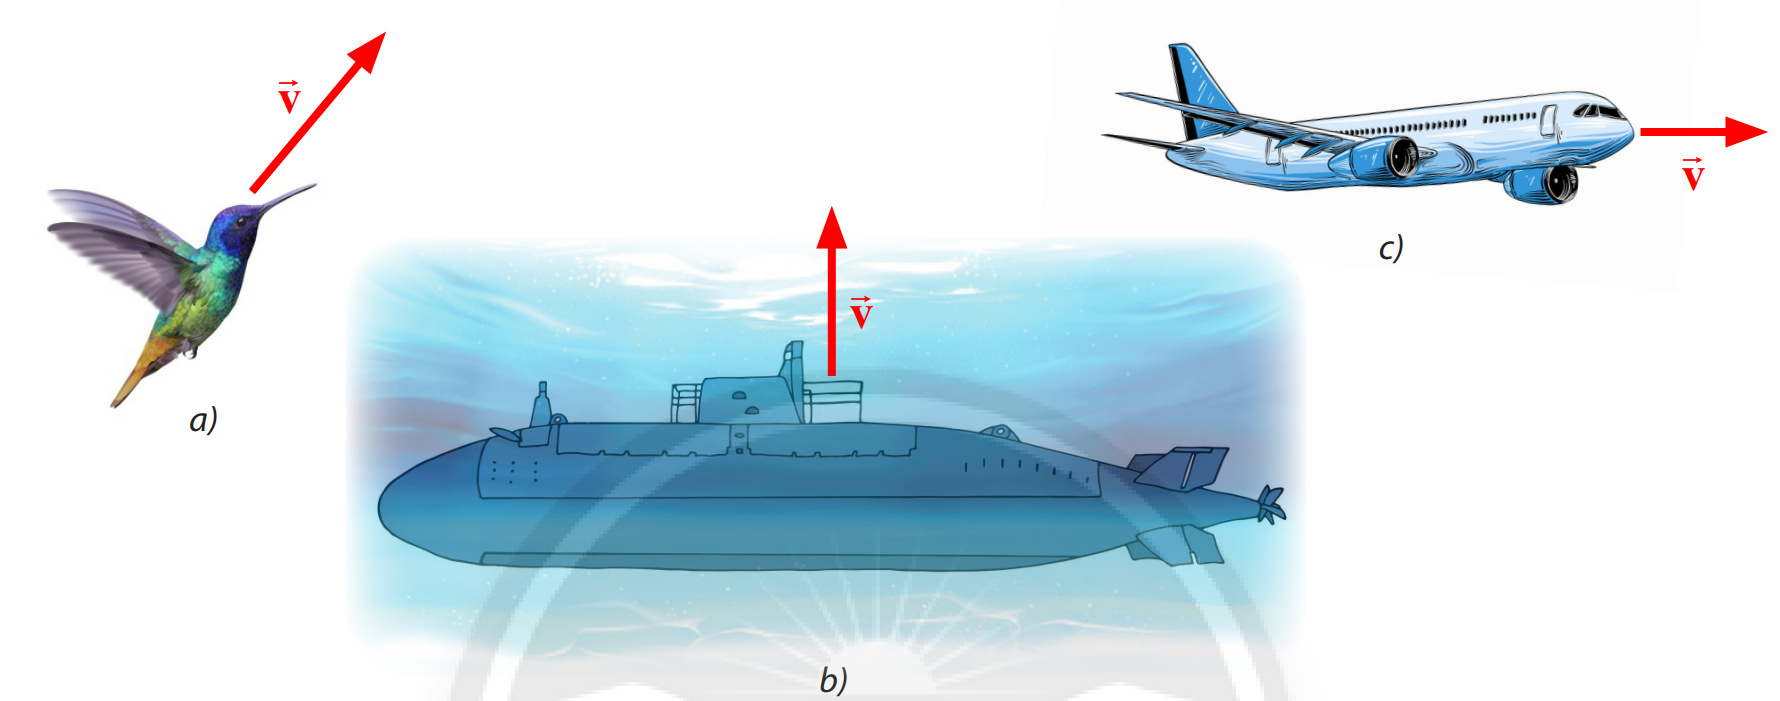
\includegraphics[width=0.6\linewidth]{../figs/VN10-2023-PH-TP020-5}
			\captionof{figure}{a) Con chim ruồi đang bay theo phương xiên hướng lên trên; b) Tàu ngầm đang di chuyển lên trên mặt nước theo phương thẳng đứng; c) Máy bay đang bay theo phương ngang.}
			\label{fig:20.5}
		\end{center}
}
{\hide{
Lực cản tác dụng lên vật được biểu diễn như hình vẽ:
\begin{center}
	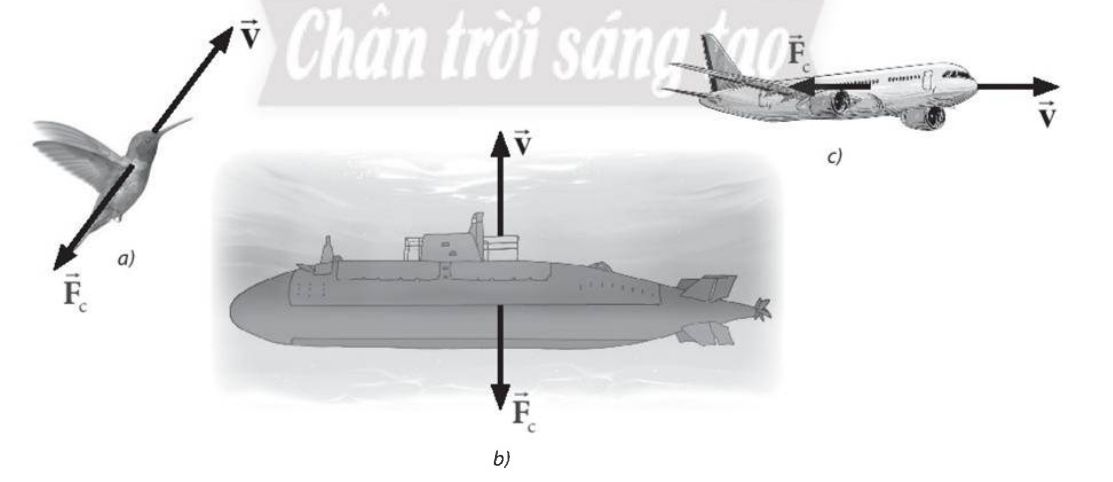
\includegraphics[width=0.6\linewidth]{../figs/VN10-2023-PH-TP020-6}
\end{center}
}}


\viduii{2}
{Một con cá hề đang bơi trong nước chịu tác dụng của lực cản $F=0,65v$ ($v$ là tốc độ tức thời tính theo đơn vị $\si{\meter/\second}$). Hãy tính lực tối thiểu để con cá đạt tốc độ $\SI{6}{\meter/\second}$, giả sử con cá bơi theo phương ngang.
	\begin{center}
		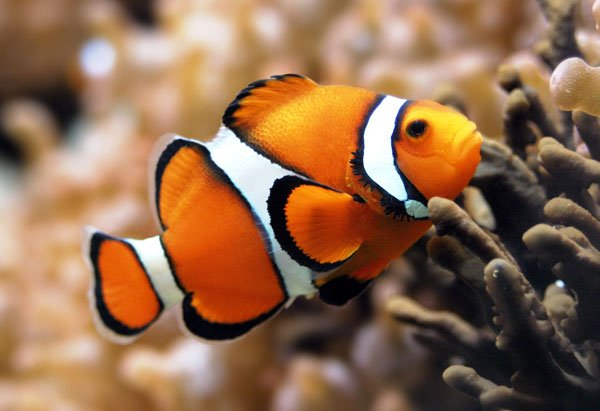
\includegraphics[width=0.2\linewidth]{../figs/VN10-2023-PH-TP020-7}
		\captionof{figure}{Cá hề}
	\end{center}
}
{\hide{
Lực tối thiểu để con cá đạt được tốc độ $\SI{6}{\meter/\second}$ là 
$$F_\text{min}=F=0,65v=0,65\cdot6=\SI{3.9}{\newton}$$
}}
\end{dang}
\begin{dang}{Giải thích được lực nâng tác dụng lên một vật ở trong trong nước (hoặc trong không khí)}
	\viduii{3}
	{\begin{minipage}[l]{0.7\textwidth}
			Một vật được móc vào lực kế như Hình \ref{fig:20.8}. Khi để ở ngoài không khí, lực kế chỉ $\SI{5}{\newton}$. Khi nhúng chìm hoàn toàn vật trong nước thì thấy lực kế chỉ $\SI{3.2}{\newton}$.
			\begin{enumerate}[label=\alph*)]
				\item Mô tả và biểu diễn các lực tác dụng lên vật.
				\item Tính lực đẩy Archimedes tác dụng lên vật.
			\end{enumerate}
		\end{minipage}
		\begin{minipage}{0.3\textwidth}
			\begin{center}
				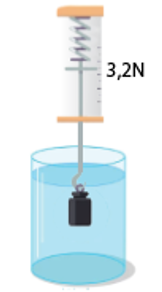
\includegraphics[width=0.3\linewidth]{../figs/VN10-2023-PH-TP020-8}
				\captionof{figure}{}
				\label{fig:20.8}
			\end{center}
		\end{minipage}
}
{\hide{
\begin{enumerate}[label=\alph*)]
	\begin{minipage}[l]{0.6\textwidth}
		\item Khi nhúng chìm hoàn toàn vật trong nước, các lực tác dụng lên vật gồm:
		\begin{itemize}
			\item Trọng lực $\vec{P}$;
			\item Lực đẩy Archimedes $\overrightarrow{F_A}$;
			\item Lực kéo của lực kế $\vec{F}$.
		\end{itemize}
	\item Khi để lực kế ngoài không khí, số chỉ của lực kế là độ lớn trọng lực của vật
	$P=\SI{5}{\newton}$.\\
	Vật nằm cân bằng trong nước:
	$$\overrightarrow{P}+\overrightarrow{F_A}+\overrightarrow{F}=\vec{0}$$
	Chiếu lên hướng của $\overrightarrow{F}$, ta có:
	$$-P+F_A+F=0\Rightarrow F_A=P-F=\SI{1.8}{\newton}$$
	\end{minipage}
	\begin{minipage}{0.4\textwidth}
		\begin{center}
			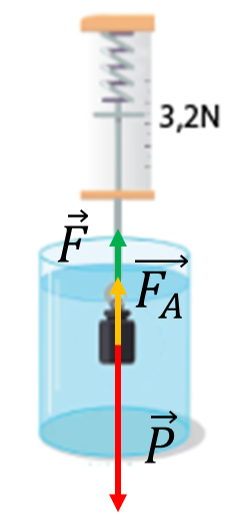
\includegraphics[width=0.3\linewidth]{../figs/VN10-2023-PH-TP020-9}
		\end{center}
	\end{minipage}

\end{enumerate}
}}

\viduii{3}
{Một khối gỗ hình hộp chữ nhật có tiết diện $S=\SI{40}{\centi\meter^2}$ cao $h=\SI{10}{\centi\meter}$. Khối gỗ có khối lượng $m=\SI{160}{\gram}$. Thả khối gỗ vào nước, khối gỗ nổi lơ lửng trên mặt nước như hình \ref{fig:20.10}. Khối lượng riêng của nước là $\rho=\SI{1000}{\kilogram/\meter^3}$. Tìm chiều cao của phần gỗ nổi trên mặt nước.
	\begin{center}
		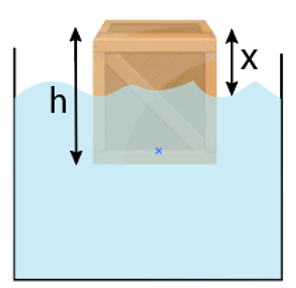
\includegraphics[width=0.2\linewidth]{../figs/VN10-2023-PH-TP020-10}
		\captionof{figure}{}
		\label{fig:20.10}
	\end{center}
}
{\hide{
Gọi $x$ là chiều cao phần khối gỗ nhô ra khỏi mặt nước, khi đó chiều cao phần khối gỗ chìm trong nước là $\left(h-x\right)$.\\
Thể tích phần gỗ chìm trong nước
$$V=S\left(h-x\right)$$
Khi khối gỗ cân bằng trong nước thì trọng lực của khối gỗ cân bằng với lực đẩy Archimedes
$$P=F_A\Leftrightarrow mg=\rho gV=\rho g S\left(h-x\right)$$
$$\Rightarrow x=h-\dfrac{m}{\rho S}=\left(\SI{0.1}{\meter}\right)-\dfrac{\left(\SI{0.16}{\kilogram}\right)}{\left(\SI{1000}{\kilogram/\meter^3}\right)\cdot\left(\SI{40E{-4}}{\meter^2}\right)}=\SI{0.06}{\meter}=\SI{6}{\centi\meter}.$$
}}
\end{dang}